\documentclass{article}
\usepackage{hyperref}
\usepackage[margin=0.5in]{geometry}
\usepackage{amsmath}
\usepackage{graphicx}
\usepackage[bottom]{footmisc}
\usepackage{lastpage}
\usepackage{fancyhdr}
\usepackage{float}
\usepackage{tabularx}

\graphicspath{ {./assets/} }

\pagestyle{fancy}
\fancyhf{} % clear existing header/footer entries
% Place Page X of Y on the right-hand
% side of the footer
\fancyfoot[R]{Yang \thepage \hspace{1pt} of \pageref{LastPage}}
\renewcommand{\headrulewidth}{0pt}

\title{PHYSIOL 578: HW 3.2\footnotetext{U-M GPT was used to help draft and refine the answers.}}
\author{Jack Yang \\ \href{mailto:yhyunjoo@umich.edu}{yhyunjoo@umich.edu}}

\begin{document}
\maketitle
\thispagestyle{fancy}

\section{
Assume that a “skinned” (definition provided in figure) skeletal muscle fiber is bathed in a
solution containing calcium but initially no ATP. Use your knowledge of the cross-bridge cycle
to answer the following questions related to the experimental record shown in the figure.
}

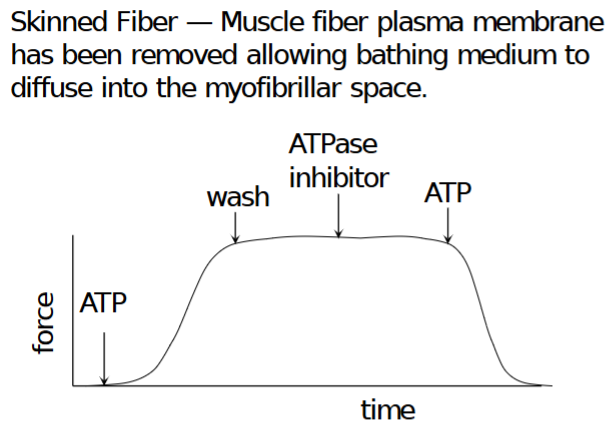
\includegraphics[width=0.5\linewidth]{fig1.png}

\subsection{
Why is there initially no force?
}
Initially, no active force is generated because ATP is unavailable to detach and energize myosin heads for force-producing cross-bridge cycling, despite the presence of Ca2+.

\subsection{
Why does force increase after ATP is
added to the bath?
}
Added ATP allows myosin to detach from actin and become energized by ATP hydrolysis. The energized heads rebind actin and undergo force-generating power strokes, increasing tension.

\subsection{
Why does force remain high when the ATP
is washed away?
}
Force remains high because ATP is required for myosin to detach from actin. When ATP is washed away, the attached cross-bridges become locked in a rigor state and maintain the existing tension.


\subsection{
Why does force remain high when an
ATPase inhibitor (prevents ATP hydrolysis) is
added to the bath?
}
Force remains high because ATP was previously washed away, leaving myosin cross-bridges attached to actin in a rigor state. Adding an ATPase inhibitor does not cause these cross-bridges to detach, so they continue to maintain the previously generated tension. Detachment requires ATP binding, not ATP hydrolysis.

\subsection{
Why does force decline when ATP is added
to the bath (the ATPase inhibitor is still
present)?
}
Force declines because ATP binds to myosin, reducing its affinity for actin and causing the rigor cross-bridges to detach. ATP binding does not require hydrolysis. However, the ATPase inhibitor prevents ATP hydrolysis, so myosin cannot become re-energized for subsequent force-producing power strokes. Thus, the existing tension is released without new force being generated.

\section{
Based on your knowledge of muscle contraction and using the cross-bridge cycle as the basis
for your answer, explain the phenomenon of rigor mortis (the temporary stiffening of the
body's muscles that occurs after death).
}
After death, ATP production stops and existing ATP is depleted. ATP-dependent Ca2+ pumps can no longer maintain low cytosolic Ca2+, allowing Ca2+ to accumulate and expose myosin-binding sites on actin. Myosin heads bind actin, but without ATP they cannot detach, leaving cross-bridges locked in a rigor state and causing muscle stiffness.


\section{
The neurotransmitter that is responsible for “communication” at the neuromuscular junction
between motor neurons and skeletal muscle fibers is acetylcholine (ACh). An action potential
in the motor neuron triggers the release of ACh, which diffuses across the small gap between
the neuron and the muscle fiber and binds to its receptor on the muscle fiber membrane. The
ACh receptor protein is a channel that opens when ACh binds. Upon the opening of this
channel, the membrane at the motor end plate region of the muscle cell becomes depolarized,
resulting in the generation of an action potential in the muscle fiber membrane.
}

\subsection{
The ACh receptor channel is \textbf{equally} permeable to both Na+ and K+ ions. Explain how
opening of this channel that increases the permeability to both potassium and sodium to
cross the membrane results in membrane depolarization.
}
Because of the differences in the ion gradients of Na+ and K+, even though Na+ is into the cell and K+ is going out,
there is more Na+ coming in than K+ going out (i.e. the reversal potential is higher than the resting potential).

\subsection{
\underline{In normal individuals}, the following is a true statement: A single end-plate potential (EPP)
is always sufficient to elicit an action potential (and hence contraction) in a skeletal-muscle
fiber. This is not the case, however, in individuals suffering from myasthenia gravis (MG,
from Greek mys plus asthenia: muscle weakness). MG is an autoimmune disorder that
affects ~1 in 20,000 individuals, in which antibodies are produced that attack the AChRs at
skeletal-muscle endplates reducing their number. Clinically, patients present with significant
muscle weakness. Explain why patients lacking sufficient numbers of AChR may exhibit
muscle weakness.
}
With fewer functional ACh receptors, the same amount of released ACh produces a smaller increase in end-plate conductance and less net inward current.
This generates a smaller end-plate potential, which may fail to depolarize the nearby muscle membrane to the threshold for activating voltage-gated Na+ channels.
Consequently, some nerve impulses fail to trigger muscle action potentials, Ca2+ release, and contraction.
Fewer muscle fibers contract successfully, resulting in muscle weakness.

\subsection{
Treatments strategies for myasthenia gravis including thymectomy (removing the source of
the antibody producing cells) and immunosuppressant drug therapy (inhibiting the
synthesis and release of the antibodies) are of limited effectiveness; however, the drug
neostigmine administered at carefully monitored doses is highly effective in treating
myasthenia gravis. Investigate the actions of \underline{neostigmine}, and discuss in detail why it is
effective in restoring neuromuscular transmission.
}
Neostigmine reversibly inhibits acetylcholinesterase, the enzyme that normally rapidly breaks down acetylcholine (ACh) in the neuromuscular junction.
Consequently, released ACh remains in the synaptic cleft longer and has more opportunities to bind and activate the remaining functional ACh receptors.

This increases the magnitude and duration of the end-plate current.
At the resting membrane potential, ACh receptor activation produces a net inward positive current, primarily through Na+ entry, generating a larger and longer-lasting end-plate potential.
This improves the likelihood of reaching the threshold for voltage-gated Na+ channel activation, restoring muscle action potentials, Ca2+ release, and contraction.

Neostigmine therefore compensates for reduced receptor numbers, but does not replace the receptors or treat the underlying autoimmune process.
Dosing must be carefully controlled because excessive ACh can cause persistent depolarization, receptor desensitization, and worsening weakness, as well as other cholinergic effects.

\end{document}